\documentclass[a4paper,12pt]{article}
\usepackage{polski}
\usepackage[utf8]{inputenc}
\usepackage{amsmath}
\usepackage{graphicx}
\usepackage{float}
\usepackage{hyperref}
\usepackage{subfig}

\usepackage{geometry}
    \geometry{
    a4paper,
    total={170mm,257mm},
    left=20mm,
    top=20mm,
}

\title{\textbf{Sprawozdanie z projektu} \\ Teoria i Metody Optymalizacji}
\author{Patrycja Kiełbasa \\ Kamil Kiełbasa}
\date{Maj 2021}

\begin{document}
\maketitle
\tableofcontents

\newpage
\section{Opis teoretyczny projektu}
\subsection{Zadanie optymalizacji}
Celem zadania jest znalezienie minimum funkcji $f(x)$ nieliniowej, ciągłej na zbiorze ograniczeń X, dla wymiaru danych $n \leq 5, m \leq 5$ w postaci:

\begin{equation} \label{eq:1}
X = [x: g_i(x) \leq 0, \quad m = 1, ... , 5]
\end{equation}

Za metodę rozwiązania została przyjęta metoda \textit{\textbf{Powella-Gaussa-Seidela}}. Natomiast za metodę minimum w kierunku została wybrana metoda \textit{\textbf{Złotego Podziału}}.

\subsection{Szczegółowe omówienie algorytmu optymalizacji}
Metoda  \textit{\textbf{Powella-Gaussa-Seidla}} z metodą minimum w kierunku  \textit{\textbf{Złotego Podziału}} to algorytmy optymalizacji lokalnej. W celu dokładnego omówienie powyższych metod należy rozbić je na trzy osobne tematy:

\begin{enumerate}
    \item Metoda przesuwanej funkcji kary Powella.
    \item Minimalizacja funkcji metodą Gaussa-Seidela.
    \item Minimalizacja w kierunku metodą Złotego Podziału.
\end{enumerate}

\subsubsection{Metoda przesuwanej funkcji kary Powella}
Istotą metody jest poszukiwanie ekstremum warunkowego przez ciąg kolejnych minimalizacji bezwarunkowych zmodyfikowanej funkcji celu. Jednakże po przekroczeniu ograniczeń lub też zwiększaniu dokładności obliczeń powiększana była stromość funkcji kary. Powodowało to niekorzystny efekt "rowu", którego skutkiem było zwiększony nakład obliczeń numerycznych. Dla złagodzenia tego zjawiska Powell zaproponował "przesuwanie" funkcji kary w trakcie procesu obliczeń, przy czym przesunięcie to uzależnił od wartości przekroczonych ograniczeń \cite{bibitem1}. Stąd też, przyjęto następującą postać modyfikacji funkcji celu:

\begin{equation} \label{eq:2}
    F(\underline{x}, \underline{\sigma}, \underline{\theta}) = f(\underline{x}) + \sum_{i=1} \sigma_{i}(g_{i} + \theta_{i})^{2} * H(g_{i} + \theta_{i})
\end{equation}

gdzie:
\begin{equation} \label{eq:3}
    \begin{split}
        \sigma_{i} > 0, \quad \underline{\sigma} = [\sigma_{1}, \sigma_{2}, ..., \sigma_{m}]^{T} &- \mbox{jest wektorem współczynników kary,} \\
        \theta_{i} > 0, \quad \underline{\sigma} = [\theta_{1}, \theta_{2}, ..., \theta_{m}]^{T} &- \mbox{wektorem przesunięć kary,}
    \end{split}
\end{equation}

oraz funkcja H, która jest funkcja skokową Heaviside’a:

\begin{equation} \label{eq:4}
    H(g_{i} + \theta_{i}) =
    \begin{cases}
        1 & \text{dla} \quad g_{i}(\underline{x}) + \theta_{i} > 0 \\
        0 & \text{dla} \quad g_{i}(\underline{x}) + \theta_{i} \leq 0
    \end{cases}
\end{equation}

\newpage
Przebieg algorytmu został przedstawiony za pomocą schematu blokowego, który pomaga zrozumieć metodę przesuwanej funkcji kary:

\begin{figure}[H]
    \centering
    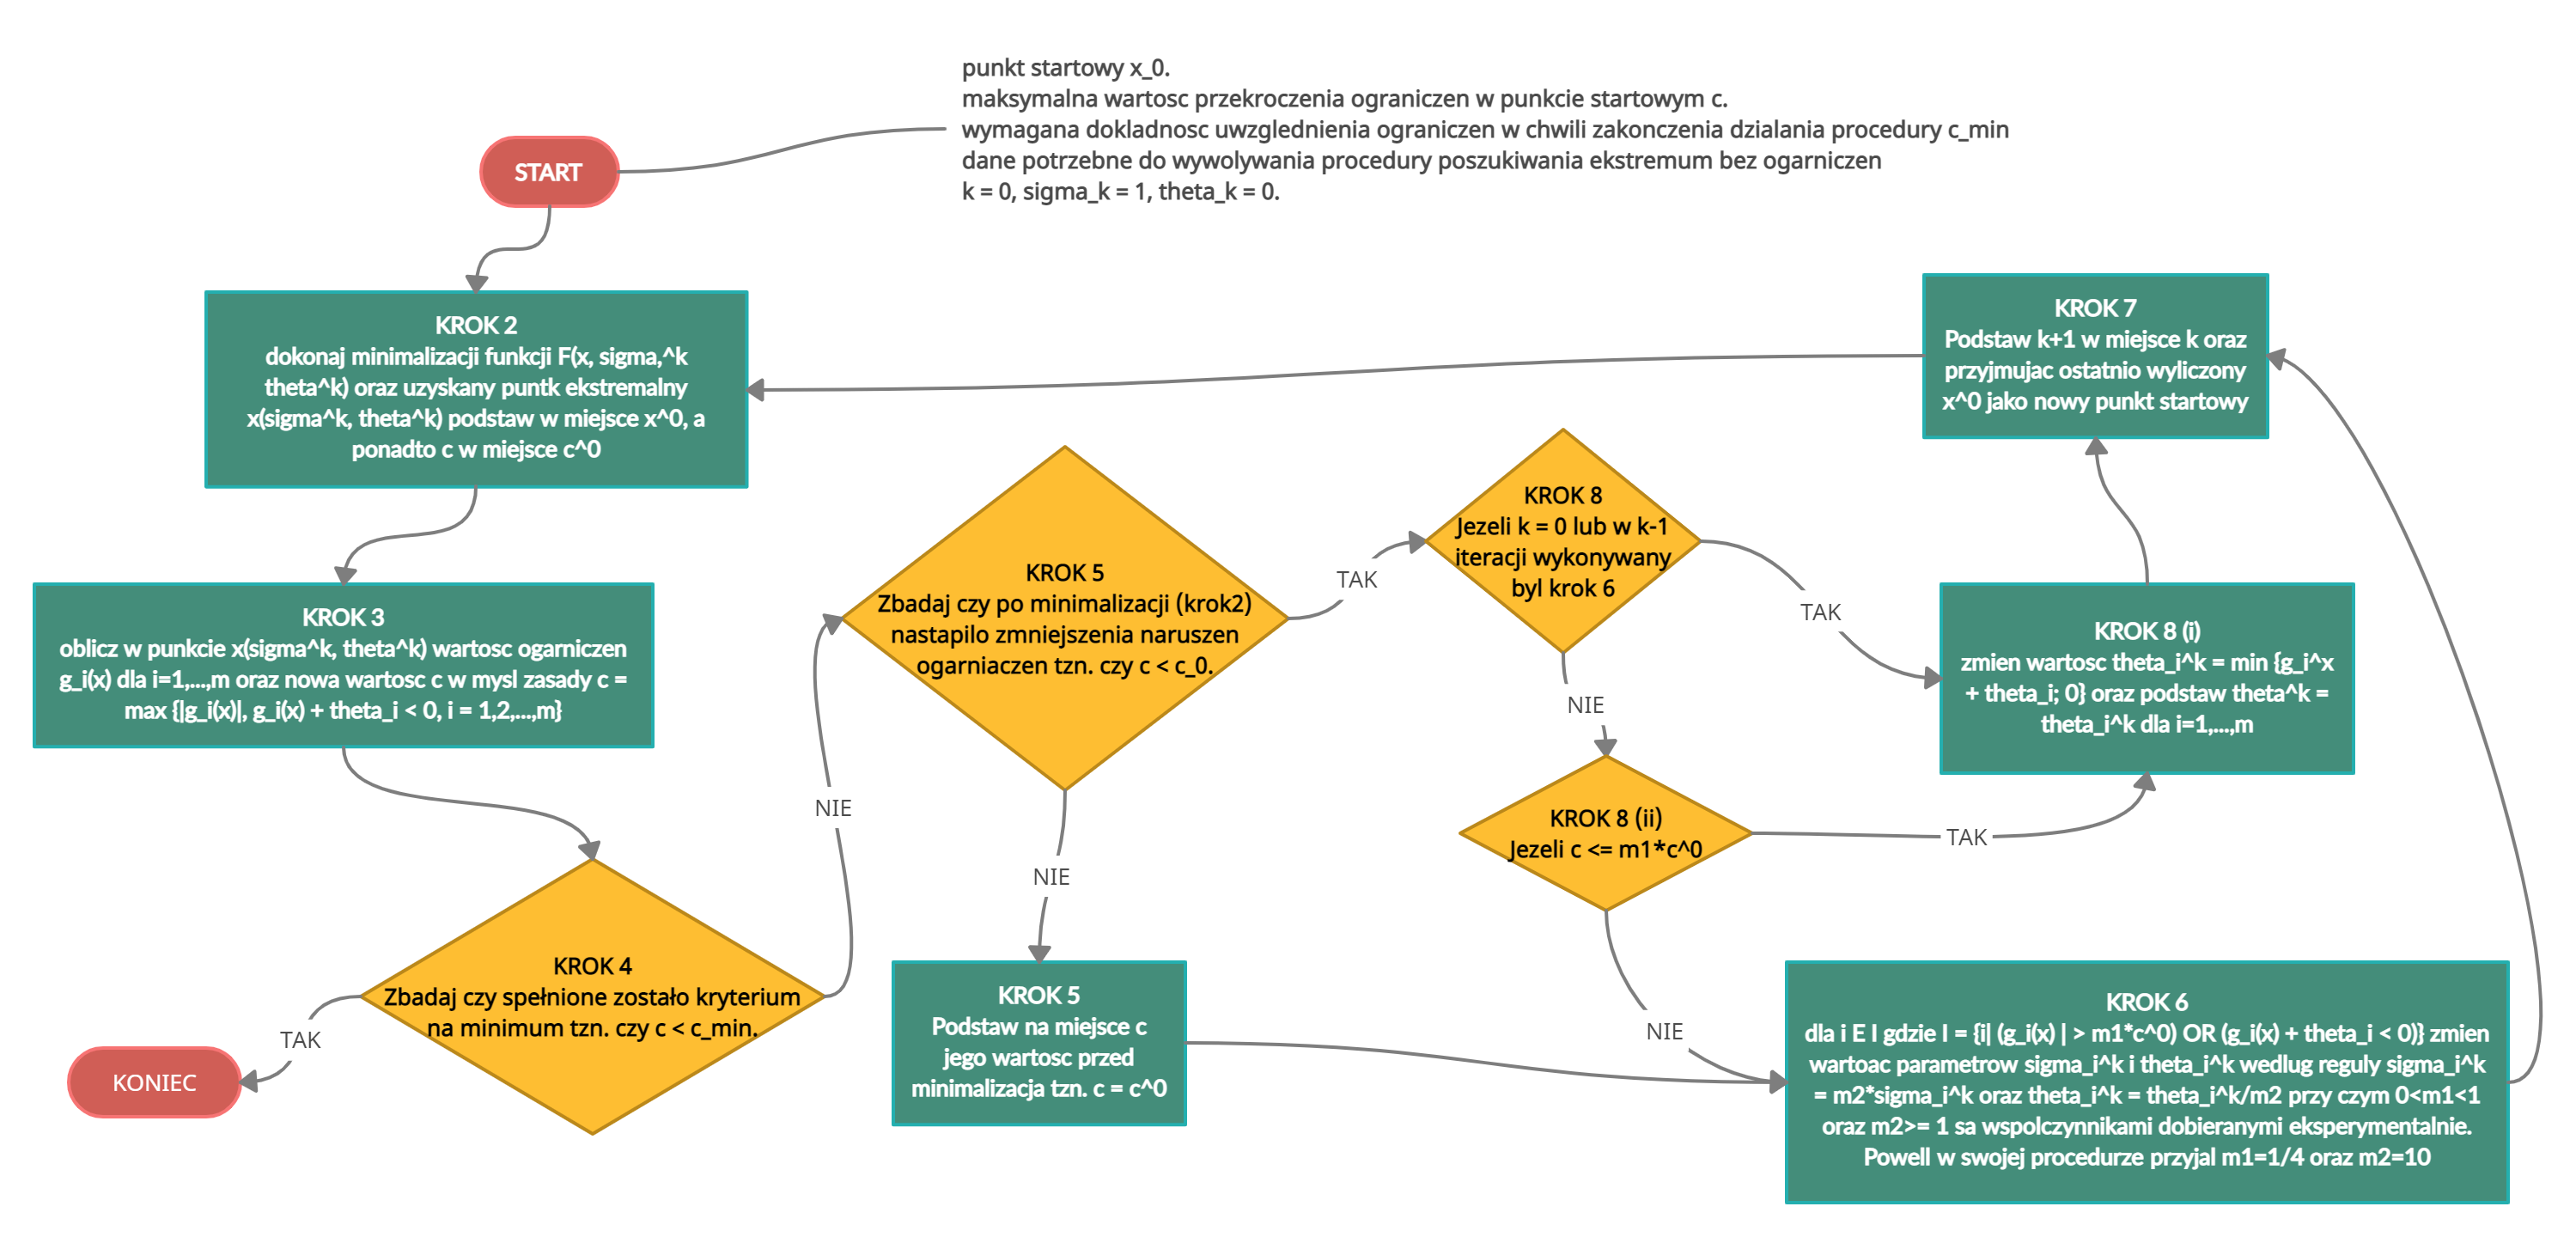
\includegraphics[width=\textwidth]{images/uml_powell.png}
    \caption{Schemat blokowy przesuwanej funkcji kary Powella.}
    \label{uml_powell}
\end{figure}

Jedynym kryterium stopu przyjętym w metodzie przesuwanej funkcji kary Powella jest minimalna wartość parametru $c$, który jest obliczany na nowo w każdej kolejnej iteracji (strona \pageref{uml_powell}, krok 3).

\begin{equation} \label{eq:5}
    c_{min} \leq \epsilon_{1}, \quad \epsilon_{1} = 10^{-1}
\end{equation}

Wartość tego parametru została domyślnie przyjęta jako $10^{-1}$, aby zmniejszyć nakład obliczeniowy. Natomiast parametr ten można dowolnie zmniejszać, aby uzyskać dokładniejszy wynik.

\subsubsection{Minimalizacja funkcji metodą Gaussa-Seidela}
Istotą metody Gaussa-Seidela jest minimalizacja funkcji $f(\underline{x})$ wzdłuż kolejnych kierunków ortogonalnej bazy $\xi_{1}, \xi_{2}, ... , \xi_{n}$, która utworzona jest z wersorów układu współrzędnych kartezjańskich \cite{bibitem1}\cite{bibitem3}. \newline

Informacje wejściowe:
\begin{align*}
    \underline{x}_{0} &- \mbox{arbitralnie wybrany punkt startowy,} \\
    \xi_{1}, \xi_{2}, ... , \xi_{n} &- \mbox{baza wyjściowa utworzona z wzajemnie ortogonalnych wektorów,} \\
    e_{0} &- \mbox{początkowa długość kroku,} \\
    \epsilon_{j} &- \mbox{wymagana dokładność obliczeń minimum w j-tym kierunku,} \\
    L &- \mbox{maksymalna liczba iteracji,} \\
    n &- \mbox{liczba zmiennych niezależnych.}
\end{align*}

\newpage
Przebieg algorytmu został przedstawiony za pomocą schematu blokowego który pomaga zrozumieć minimalizację funkcji metodą Gaussa-Seidela:
\begin{figure}[H]
    \centering
    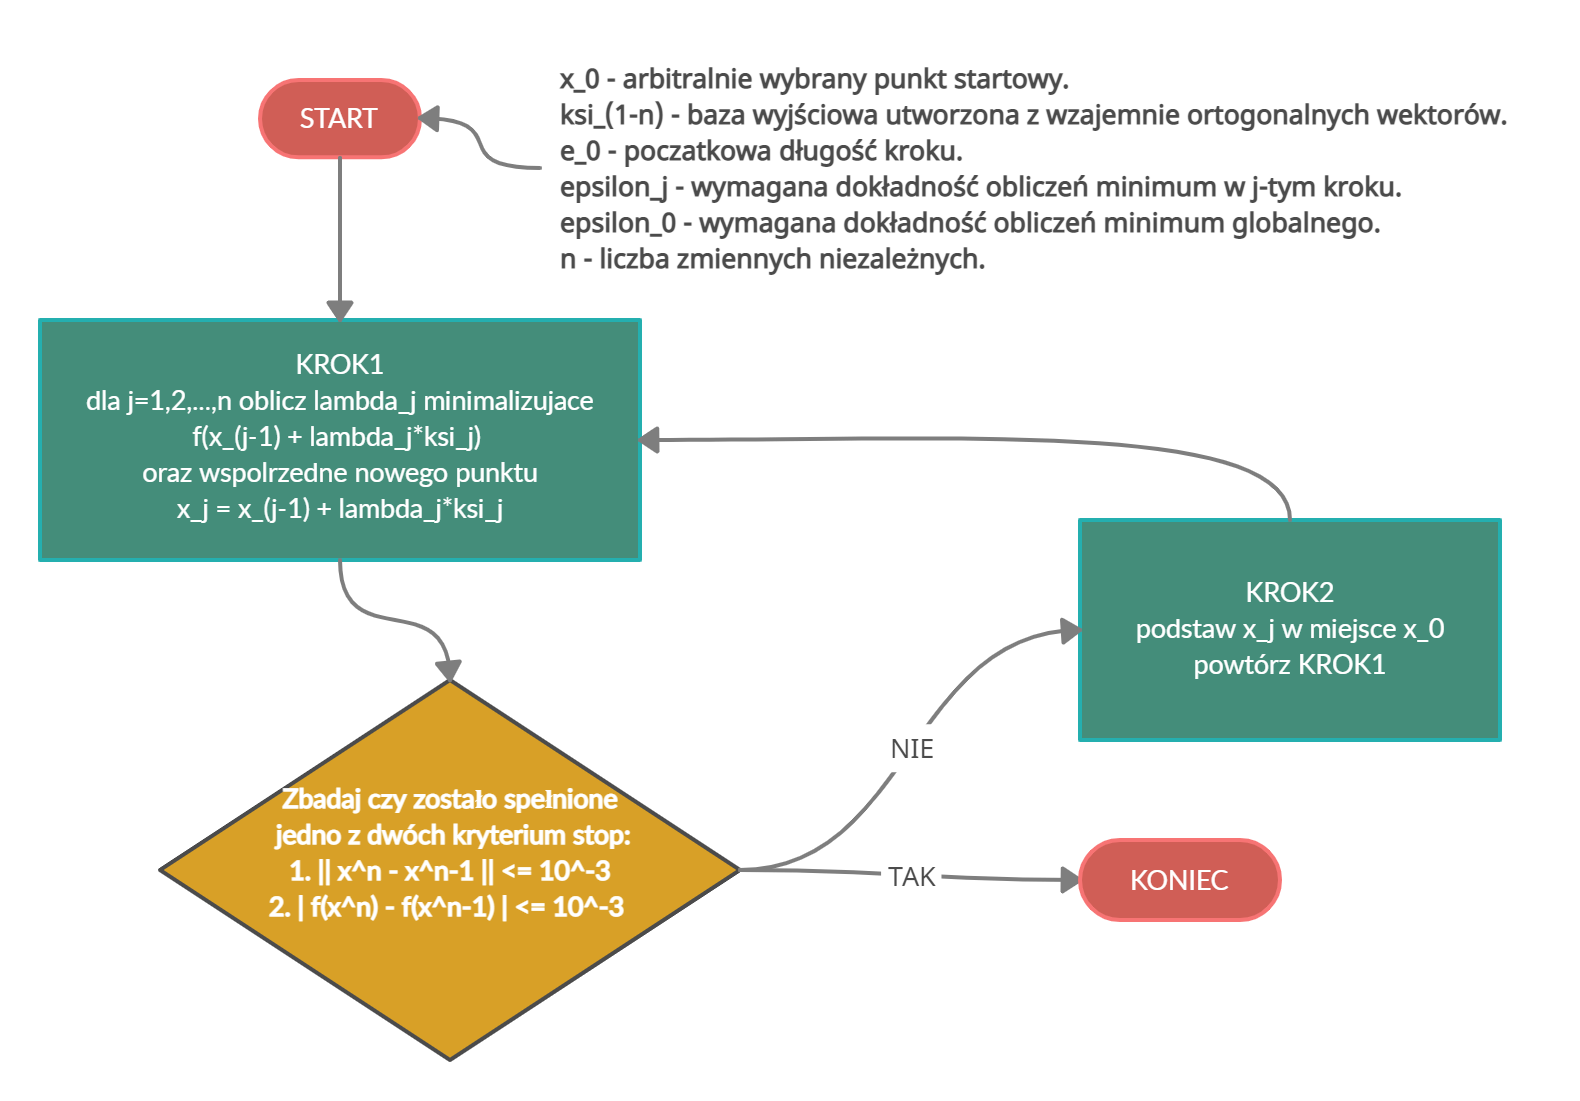
\includegraphics[width=\textwidth]{images/uml_gauss_seidel.png}
    \caption{Schemat blokowy dla minimalizacji funkcji metodą Gaussa-Seidela.}
    \label{uml_gauss_seidel}
\end{figure}

W przypadku metody Gaussa-Seidela zostały przyjęte następujące trzy kryteria stopu:
\begin{equation} \label{eq:6}
    \begin{split}
        || x^{n} - x^{n-1} || &\leq \epsilon_{2}, \quad \epsilon_{2} = 10^{-3} \\
        | f(x^{n}) - f(x^{n-1}) | &\leq \epsilon_{3}, \quad \epsilon_{3} = 10^{-3} \\
        L &= 1000
    \end{split}
\end{equation}

Algorytm zakończy swoje działanie w trzech przypadkach:
\begin{enumerate}
    \item Różnica odległości pomiędzy obecnym a nowo znalezionym punktem jest mniejsza niż $\epsilon_{2}$.
    \item Różnica wartości minimalizowanej funkcji celu, pomiędzy obecnym a nowo znalezionym punktem jest mniejsza niż $\epsilon_{3}$.
    \item Przekroczona zostanie maksymalna liczba iteracji.
\end{enumerate}

\newpage
\subsubsection{Minimalizacja w kierunku metodą Złotego Podziału}
Jako metoda minimalizacji w kierunku została wybrana metoda Złotego Podziału która jest jedną z najczęściej stosowanych metod służących do zawężania przedziału poszukiwań. Idea metody oparta jest na założeniu, że w każdym kroku obliczeń długość przedziału poszukań zmniejszany jest w stałym stosunku $\alpha = \frac{\sqrt{5} - 1}{2}$ \cite{bibitem2}. Metoda ta została wybrana ze względu na prostotę algorytmu, co przekłada się na łatwą implementację. Istnieje również wiele sprawdzonych źródeł wiedzy wraz z gotowymi przykładami jak i ich wizualnym opisem, na podstawie których można testować poprawność metody \cite{bibitem1}\cite{bibitem2}. \newline

Informacje wejściowe:
\begin{align*}
    x &- \mbox{punkt początkowy,} \\
    [a^{(i)}, b^{(i)}] &- \mbox{przedział poszukiwań,} \\
    \xi &- \mbox{kierunek poszukiwań,} \\
    \epsilon &- \mbox{dokładność rozwiązania,} \\
    L &- \mbox{maksymalna liczba iteracji.}
\end{align*}

Kryterium stopu:
\begin{equation} \label{eq:7}
    \begin{split}
        \epsilon &- \mbox{pożądana dokładność przedziału [a, b],} \\
        L &- \mbox{maksymalna liczba iteracji.}
    \end{split}
\end{equation}

\subsubsection{Zasada działania Powella, Gaussa-Seidela i Złotego Podziału}
Na podstawie wcześniej opisanych oddzielnie metoda, możemy przejść do wytłumaczenia działania całości algorytmu jako zbioru kilku metod w bardzo ogólny oraz uproszczony sposób:

\begin{enumerate}
    \item Zakładamy, że do metod zostały przekazane wszystkie wymagane informacje wstępne.
    \item W metodzie przesuwanej funkcji Powella sprawdzamy, czy nie został spełniony warunek stopu, równanie numer \ref{eq:5}. Jeżeli tak to kończymy działanie całej procedury.
    \item Jeżeli nie, to dokonujemy minimalizacji zmodyfikowanej funkcji celu a funkcję przesuwanej kary (równanie numer \ref{eq:2}) za pomocą metody Gaussa-Seidela, generując w ten sposób nowy punkt.
    \item Wewnątrz metody Gaussa-Seidela, dokonujemy minimalizacji w n-kierunkach za pomocą metody minimum w kierunku Złotego Podziału.
    \item Metoda Złotego Podziału zawęża przedział poszukiwań do wymaganej dokładności lub do maksymalnej liczby iteracji, opisanymi warunkami numer \ref{eq:7}.
    \item Metoda Gaussa-Seidela poszukuje nowych punktów aż do momentu spełnienia kryteriów stopu, opisanych warunkami numer \ref{eq:6}.
    \item Po zakończeniu procedury Gaussa-Seidela, w metodzie Powella następuje przesuwanie kary, poprzez odpowiednie modyfikowanie wektorów $\theta, \sigma$. Schemat postępowania opisany jest przez schemat blokowy na stronie numer \pageref{uml_powell} (kroki 3-8).
    \item Wracamy do punktu drugiego.
\end{enumerate}


\section{Informacje ogólne o programie}
Zanim została podjęta decyzja o wyborze środowiska programistycznego, zostało przeanalizowane kilka języków oraz bibliotek, które dla danego języka są dostępne. Rozważane były następujące środowiska programistyczne: \textit{.NET}, \textit{Matlab} oraz \textit{Python}. Finalnie zdecydowaliśmy się wybrać \textit{Python} jako środowisko programistyczne ze względu na mnogość oraz bogactwo bibliotek, jak i prostotę używania. Warunkiem koniecznym do wyboru środowiska programistycznego było posiadanie przez środowisko bibliotek, które umożliwiają następujące operacje: 
\begin{itemize}
    \item parsowanie równań oraz obliczanie ich wartości.
    \item efektywne operacje na wektorach i macierzach.
    \item rysowanie wykresów i możliwość nanoszenie dodatkowych elementów (punkty, funkcje).
    \item tworzenie interfejsu użytkownika.
\end{itemize} 

\begin{flushleft}
    Biblioteki, które zostały wykorzystane do implementacji projektu:
\end{flushleft}

\begin{itemize}
    \item \textbf{sympy} - biblioteka ta jest szeroko opisana poprzez bogatą dokumentację oraz jest przedstawiana na wielu uczelniach, na kierunkach matematycznych. Umożliwia ona obliczenia wielu skomplikowanych równań (wielomiany, sumy, iloczyny, całki, równania różniczkowe), posiada wbudowany parser, który potrafi przekształcić równanie z formy tekstowej na formę, która umożliwią obliczenia wartości ten funkcji przez bibliotekę. Jako plus warto wymienić, iż biblioteka ta kładzie duży nacisk na dokładność numeryczną względem innych bibliotek.
    \item \textbf{numpy} - biblioteka ta dostarcza odpowiednich narzędzi do wszelkich operacji na wektora i macierzach. Jest odpowiednio zoptymalizowana względem Pythona więc stosowanie np. list zamiast wektorów z bibliteki numpy bardzo zwalniałoby wykonywanie się programu.
    \item \textbf{matplotlib} - w Matlabie tworzenie wykresów jest wręcz czymś naturalnym. Funkcjonalność ta została z Matlaba przeniesiona wprost do Pythona, dzięki czemu biblioteka ta umożliwia szeroką paletę możliwości tworzenia różnego rodzaju wykresów jak np. tworzenie warstwic, nanoszenie ograniczeń, rysowanie kolejnych kroków algorytmów czy możliwość powiększania/pomniejszania wykresów w celu analizy uzyskanych wyników.
    \item \textbf{tkinter} - biblioteka ta umożliwia proste i bardzo szybkie tworzenie interfejsu. Jest bardzo podobna do szeroko znanego frameworku Qt lub Windows Form, dzięki czemu dla wielu wykorzystanie tej biblioteki będzie czymś naturalnym ze względu na duże podobieństwo. Minusem biblioteki jest bardzo słabo opisana dokumentacja natomiast ze względu na wiek frameworku do tego czasu powstało wiele poradników, które stanowią dobre źródło wiedzy.
\end{itemize}

\subsection{Wygląd aplikacji oraz funkcjonalność}
\begin{figure}[H]
    \centering
    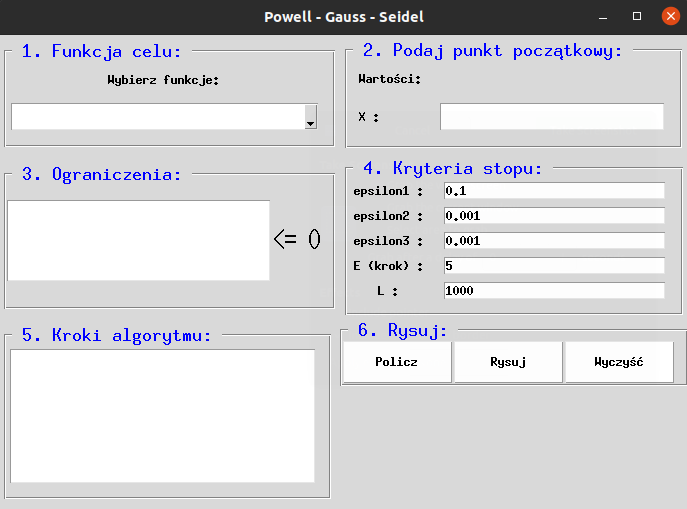
\includegraphics[width=\textwidth]{images/timo_aplikacja.png}
    \caption{Wizualny wygląd aplikacji.}
    \label{uml_gauss_seidel}
\end{figure}

\begin{flushleft}
    Opis funkcjonalności:
\end{flushleft}

\begin{enumerate}
    \item \textbf{Funkcja celu} - okno to pozwala na wybór już wprowadzonych do aplikacji funkcji celu, jak i do dodania nowej, dlatego pasek domyślnie jest pusty.
    \item \textbf{Podaj punkt początkowy} - okno to pozwala na podanie dowolnego punktu początkowego. Każdą kolejną wartość punktu początkowego należy oddzielić za pomocą średnika.
    \item \textbf{Ograniczenia} - w przypadku tego okna istnieją dwie możliwości: \textit{puste} lub \textit{wypełnione}. Jeżeli okno to zostanie puste, domyślanie zostanie uruchomiony algorytm Gaussa-Seidela dla zadania programowania nieliniowego bez ograniczeń. Natomiast po wpisaniu minimum jednego ograniczenia, domyślanie zostanie uruchomiony algorytm Powella-Gaussa-Seidela dla zadania programowania nieliniowego z ograniczeniami.
    \item \textbf{Kryteria stopu} - okno to pozwala modyfikować parametry wejściowe do obu metod:
        \begin{itemize}
            \item \textit{epsilon1} - parametr ten jest związany z metodą Powella i został opisany równaniem numer \ref{eq:5}.
            \item \textit{epsilon2, epsilon3} - parametry te są związane z dokładnością metody Gaussa-Seidela i zostały opisane równaniem numer \ref{eq:6}.
            \item \textit{E (krok)} - parametr ten definiuje długość kroku, która zostanie wykonana przez metodę Gaussa-Seidela, a w praktyce zostanie przekazana do metody minimum w kierunku jaką jest metoda Złotego Podziału.
            \item \textit{L} - parametr ten definiuje maksymalną ilość iteracji metody Gauss-Seidela oraz Złotego Podziału, tak aby uniknąć nieskończonego wykonywania się programu.
        \end{itemize}
    \item \textbf{Kroki algorytmu} - okno to będzie wyświetlać kolejne iteracje dla algorytmów w następującym formacie (w zależności czy zostaną podane ograniczenia) :
        \begin{itemize}
            \item \textit{Powell-Gauss-Seidel} - zostanie wypisany punkt, wartość funkcji celu dla tego punktu oraz wartość parametru $\epsilon$ opisanego warunkiem numer \ref{eq:5}.
            \item \textit{Gauss-Seidel} - zostanie wypisany punkt oraz wartość funkcji celu dla tego punktu.
        \end{itemize}
    \item \textbf{Rysuj} - okno to zawiera trzy przyciski:
        \begin{itemize}
            \item \textit{Policz} - przycisk ten uruchamia tylko i wyłączanie obliczenia, które znajdą się pod oknem numer 5 $\rightarrow$ \textit{Kroki algorytmu}.
            \item \textit{Rysuj} - przycisk ten w przypadku zadania nieliniowego dla $n = 2$ wyrysuje odpowiednio warstwicę, ograniczenia jeżeli zostały podane oraz kolejne kroki algorytmu.
            \item \textit{Wyczyść} - przycisk ten pozwala wyczyścić okno numer 5 $\rightarrow$ \textit{Kroki algorytmu}.
        \end{itemize}
\end{enumerate}

\subsection{Zasady wprowadzania danych początkowych}
Dane wprowadzamy w zależności od typu danych:
\begin{itemize}
    \item \textbf{Ograniczenia} - każde z ograniczeń wprowadzamy jedno pod drugim. Zmienne, które używamy to odpowiednio $x1, x2, ..., x5$. Każdą operację mnożenia oddzielamy znakiem mnożenia. Ułamki wprowadzamy z użyciem kropki, nie przecinka.
    \item \textbf{X} - zgodnie z założeniami projektu maksymalny rozmiar zadania to $n = 5$. Każda wartość punktu początkowego powinna być liczbą całkowitą, oddzielona średnikiem.
    \item \textbf{epsilon 1,2,3} - ograniczenie decydujące o precyzji uzyskanego rozwiązania. Można przyjąć liczbę całkowita natomiast nie ma to większego sensu. Ograniczenia te to ułamki, które przedziela kropka. Warto pamiętać o tym, że im mniejsze ograniczeniami, tym algorytm będzie dłużej wykonywał obliczenia.
    \item \textbf{E (krok)} - długość kroku dla Złotego Podziału to liczba naturalna. Od wielkości tej liczby zależy czy zostanie znalezione inne minimum lokalne.
    \item \textbf{L} - liczba ta ogranicza maksymalną liczbę iteracji metod Gaussa-Seidela oraz Złotego Podziału. Jest to liczba naturalna i sugeruje się aby nie była mniejsza niż 1000 (czyli domyślna), przyjmując coraz to większe dokładności \textit{epsilon 1,2,3}.
\end{itemize}


\newpage
\section{Przykłady testowe}
\subsection{Algorytm Gaussa-Seidela}
\subsubsection{Przykład I}
Funkcja celu:
\begin{equation}
    f(x_{1}, x_{2}) = (x_{1} - 2)^{2} + (x_{2} - 1)^{2}
\end{equation}
%comment
Parametry wejściowe:
\begin{align*}
    x &= [0; 0] \\
    \epsilon_{2} &= 10^{-3} \\
    \epsilon_{3} &= 10^{-3} \\
    E &= 5 \mbox{ (długość kroku)}\\
    L &= 1000
\end{align*}
%comment
Rezultat w postaci warstwicy i zaznaczonych kolejnych kroków:
\begin{figure}[H]
    \centering
    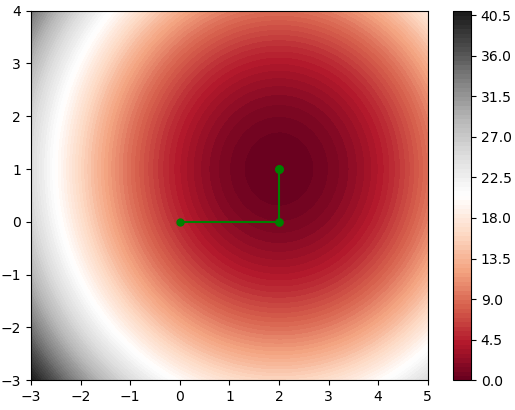
\includegraphics[width=\textwidth]{images/gs_plot1.png}
    \caption{Kolejne kroki metody Gaussa-Seidela dla powyższego przykładu.}
    \label{uml_gauss_seidel}
\end{figure}
%comment
Spis kolejnych punktów i wartości funkcji celu:
\begin{align*}
x &= [0, 0] & f(x) &= 5.00 \\
x &= [1.99976564520477, 0] & f(x) &= 1.00000005492217 \\
x &= [1.99976564520477, 0.999831752166127] & f(x) &= 8.32295036479788 * 10^{-8} \\
x &= [2.00019832088406,0.999831752166127] & f(x) &= 6.76385066555492 * 10^{-8} \\
x &= [2.00019832088406,1.00026442784541] & f(x) &= 1.09253258479443 * 10^{-7}
\end{align*}
%comment
\newline
\textbf{\textit{Szczegółowy opis techniki rozwiązania zadania:}} \\
Jest to pierwszy przykład funkcji, w której testowany był algorytm \textit{Gaussa-Seidela}. Patrząc na wykres można mieć wrażenie, iż algorytm wykonał tylko i wyłącznie dwa kroki, w prawo i do góry, natomiast ze spisu uzyskanych punktów widać że po osiągnięciu punktu $x ~= [2, 1]$, algorytm przesuwał się dalej w prawo i do góry zwiększając dokładność uzyskanego wyniku, aż do zakończenia poprzez jedno z kryteriów stopu.

\subsubsection{Przykład II}
Funkcja celu:
\begin{equation}
    f(x_{1}, x_{2}) = x_{1}^{4} + x_{2}^{4} - x_{1}^{2} - x_{2}^{2}
\end{equation}
%comment
Parametry wejściowe:
\begin{align*}
    x &= [4; 4] \\
    \epsilon_{2} &= 10^{-3} \\
    \epsilon_{3} &= 10^{-3} \\
    E &= 5 \mbox{ (długość kroku)}\\
    L &= 1000
\end{align*}
%comment
\newpage
Rezultat w postaci warstwicy i zaznaczonych kolejnych kroków:
\begin{figure}[H]
    \centering
    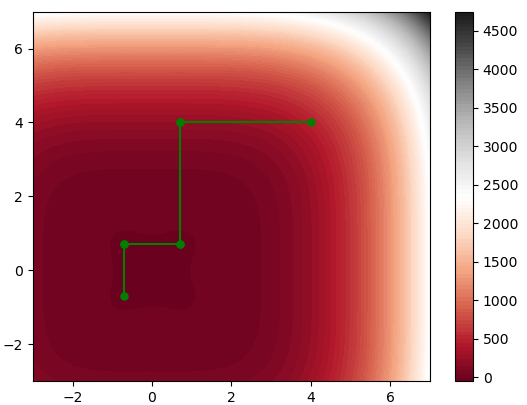
\includegraphics[width=\textwidth]{images/gs_plot2.png}
    \caption{Kolejne kroki metody Gaussa-Seidela dla powyższego przykładu.}
    \label{uml_gauss_seidel}
\end{figure}
%comment
Spis kolejnych punktów i wartości funkcji celu:
\begin{align*}
x &= [4; 4] & f(x) &= 480.00 \\
x &= [0.706997263035222, 4] & f(x) &= 239.750000023985 \\
x &= [0.706997263035222, 0.706997263035222] & f(x) &= -0.499999952030529 \\
x &= [-0.707231617830448, 0.706997263035222] & f(x) &= -0.499999944841386 \\
x &= [-0.707231617830448,-0.707231617830448] & f(x) &= -0.499999937652243 \\
\end{align*}
%comment
\newline
\textbf{\textit{Szczegółowy opis techniki rozwiązania zadania:}} \\
W przykładzie tym została przetestowana umiejętność algorytmu \textit{Gaussa-Seidela} do zmiany bazy ortogonalnej wektorów $\xi$. Domyślanie algorytm ma się poruszać w górę oraz w prawo, natomiast już w pierwszej iteracji algorytm \textit{Gaussa-Seidela} wie, że oddalałby się od minimum lokalnego, więc wykonuje kolejne ruchy w lewo oraz w dół. Algorytm znajduje kolejno trzy minima lokalne, w każdej w kolejnych iteracji zmniejszając ósme miejsce po przecinku.

\newpage
\subsubsection{Przykład III}
Funkcja celu:
\begin{equation}
    f(x_{1}, x_{2}) = (x_{1} - 2)^{2} + (x_{1} - x_{2}^{2})^{2}
\end{equation}
%comment
Parametry wejściowe:
\begin{align*}
    x &= [0; 0] & x &= [0; 0]\\
    \epsilon_{2} &= 10^{-3} & \epsilon_{2} &= 10^{-3} \\
    \epsilon_{3} &= 10^{-3} & \epsilon_{3} &= 10^{-3} \\
    E &= 2 \mbox{ (długość kroku)} & E &= 5 \mbox{ (długość kroku)}\\
    L &= 1000 & L &= 1000
\end{align*}
%comment
Rezultat w postaci warstwicy i zaznaczonych kolejnych kroków:
\begin{figure}[H]
    \centering
    \subfloat[\centering minimum pierwsze]{{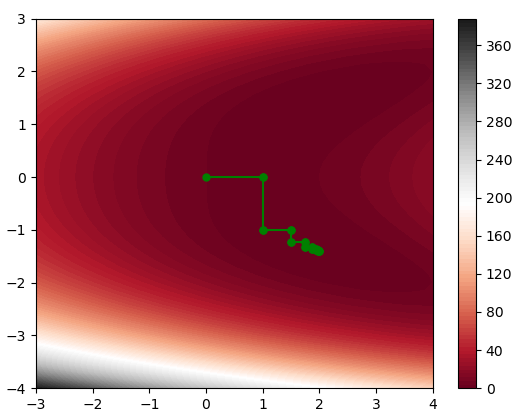
\includegraphics[width=0.47\textwidth]{images/gs_plot3_E2.png} }}%
    \quad
    \subfloat[\centering minimum drugie]{{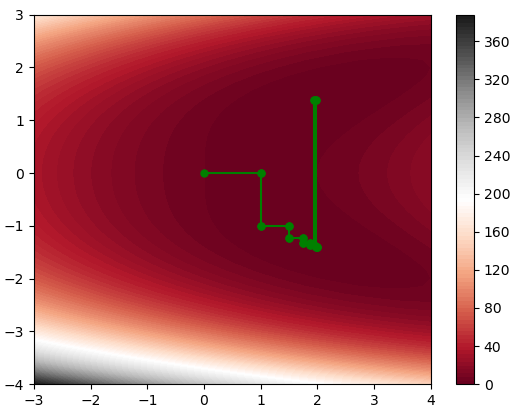
\includegraphics[width=0.47\textwidth]{images/gs_plot_E5.png} }}%
    \caption{Kolejne kroki metody Gaussa-Seidela dla powyższego przykładu.}
\end{figure}
%comment
Spis kolejnych punktów i wartości funkcji celu dla obu minimów:
\begin{align*}
x &= [0, 0] & x &= [0,0] \\
f(x) &= 4.00 & f(x) &= 4.00 \\
\hline
x &= [1.00028003358207, 0] & 
x &= [0.999831752166127, 0] \\
f(x) &= 2.00000015683761 & 
f(x) &= 2.00000005661467 \\
\hline 
x &= [1.00028003358207, -1.00028003358207] & 
x &= [0.999831752166127, -0.999831752166127] \\
f(x) &= 0.999440089717395 & 
f(x) &= 1.00033655227289 \\
\hline 
x &= [1.50008653513586, -1.00028003358207] & 
x &= [1.49996396608883, -0.999831752166127] \\
f(x) &= 0.499440086212233 & 
f(x) &= 0.500336558919113 \\
\hline 
x &= [1.50008653513586, -1.22455170514679] & 
x &= [1.49996396608883, -1.22465866845715] \\
f(x) &= 0.249913785567936 & 
f(x) &= 0.250036065873776 \\
\hline 
x &= [1.74976323398586, -1.22455170514679] & 
x &= [1.74991587608306, -1.22465866845715] \\
f(x) &= 0.125236672633066 & 
f(x) &= 0.125105596097763 \\
\hline 
x &= [1.74976323398586, -1.32257223406998] & 
x &= [1.74991587608306, -1.32279098312854] \\
f(x) &= 0.0626187593302715 & 
f(x) &= 0.0625420886048040 \\
\hline 
x &= [1.87465506506603, -1.32257223406998] & 
x &= [1.87510816891982, -1.32279098312854] \\
f(x) &= 0.0314509999326297 & 
f(x) &= 0.0313061257851012 \\
\hline 
x &= [1.87465506506603, -1.36943656787918] & 
x &= [1.87510816891982, -1.36947742422819] \\
f(x) &= 0.0157118447434279 & 
f(x) &= 0.0155980992481376 \\
\hline 
x &= [1.93778063638680, -1.36943656787918] & 
x &= [1.93765324490194, -1.36947742422819] \\
f(x) &= 0.00776802033352175 & 
f(x) &= 0.00775407088265415 \\
\hline 
x &= [1.93778063638680, -1.39201600873139] & 
x &= [1.93765324490194, 1.39190422298319] \\
f(x) &= 0.00387125440220234 & 
f(x) &= 0.00388718334529151 \\
\hline 
x &= [1.96894379984858, -1.39201600873139] & 
x &= [1.96881158592588, 1.39190422298319] \\
f(x) &= 0.00194012724121721 & 
f(x) &= 0.00195957038862184 \\
\hline 
x &= [1.96894379984858, -1.40307917723060] & 
x &= [1.96881158592588, 1.40312967845529] \\
f(x) &= 0.000964585300528995 & 
f(x) &= 0.000972718669480574 \\
\hline 
x &= [1.98419186634222, -1.40307917723060] & 
x &= [1.98444182687411, 1.40312967845529] \\
f(x) &= 0.000492032124556021 & 
f(x) &= 0.000487572190815397 \\
\hline 
x &= [1.98419186634222, -1.40883731340710] & 
x &= [1.98444182687411, 1.40862820922422] \\
f(x) &= 0.000250294883970871 & 
f(x) &= 0.000242100179512883 \\
\hline
\end{align*}
%comment
\newline
\textbf{\textit{Szczegółowy opis techniki rozwiązania zadania:}} \\
Funkcja celu w tym przypadku przypomina "nerkę" i posiada dwa minima lokalne, które powinny zostać znalezione przez algorytm \textit{Gaussa-Seidela}. Aby to osiągnąć należy najpierw zobaczyć warstwicę funkcji i odpowiednio dobrać długość kroku tak, aby wykorzystywana metoda minimum w kierunku, czyli \textit{Złoty Podział} mogła znaleźć jedno z minimów, oddalonego od drugiego. W przypadku przyjęcia długości kroku $E = 2$ (warstwica po lewej stronie) możemy zauważyć, że algorytm znajduje jedno z minimów, ale nie jest w stanie przejść do drugiego, ponieważ długość kroku mu na to nie pozwala. W drugim przypadku gdy długość kroku została zwiększona $E = 5$, możemy zauważyć, że algorytm poprawnie znalazł drugie minimum lokalne, co potwierdza wpływ zmiany długości kroku na zachowanie się algorytmu \textit{Gaussa-Seidela}.

\newpage
\subsection{Algorytm Powella-Gaussa-Seidela}
\subsubsection{Przykład I}
Funkcja celu:
\begin{equation}
    f(x_{1}, x_{2}) = (x_{1} - 2)^{2} + (x_{2} - 1)^{2}
\end{equation}
%comment
Ograniczenia:
\begin{equation}
    \begin{split}
        x_{1}^{2} - x_{2} &\leq 0 \\
        x_{1} + x_{2} - 2 &\leq 0
    \end{split}
\end{equation}
%comment
Parametry wejściowe:
\begin{align*}
    x &= [0; 0] \\
    \epsilon_{1} &= 10^{-1} \\
    \epsilon_{2} &= 10^{-3} \\
    \epsilon_{3} &= 10^{-3} \\
    E &= 5 \mbox{ (długość kroku)}\\
    L &= 1000
\end{align*}
%comment
Rezultat w postaci warstwicy i zaznaczonych kolejnych kroków:
\begin{figure}[H]
    \centering
    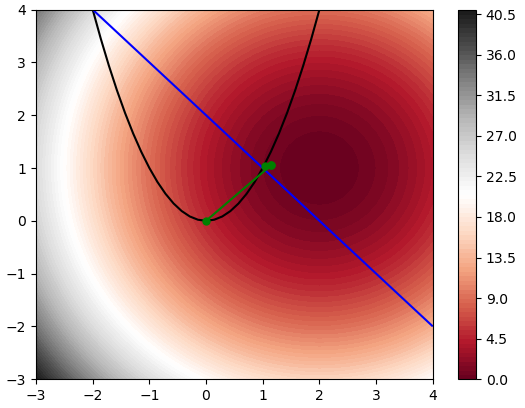
\includegraphics[width=\textwidth]{images/p_plot1.png}
    \caption{Kolejne kroki metody Powella-Gaussa-Seidela dla powyższego przykładu.}
    \label{uml_gauss_seidel}
\end{figure}
%comment
Spis kolejnych punktów, wartości funkcji celu oraz \textit{c}  dla $\epsilon_{1} = 10^{-1}$:
\begin{align*}
x &= [0, 0] & f(x) &= 5.00 & c &= 5 \\
x &= [1.15391686675790, 1.05914381664824] & 
f(x) &= 0.719354659404491 & 
c &= 0.272380318740130 \\
x &= [1.04101966249685, 1.03401882294503] & 
f(x) &= 0.920800568032229 & 
c &= 0.0750384854418764 
\end{align*}
%comment
Spis kolejnych punktów, wartości funkcji celu oraz \textit{c}  dla $\epsilon_{1} = 10^{-3}$:
\begin{align*}
x &= [0, 0] & f(x) &= 5.00 & c &= 5 \\
x &= [1.15391686675790, 1.05914381664824] & 
f(x) &= 0.719354659404491 & 
c &= 0.272380318740130 \\
x &= [1.04101966249685,1.03401882294503] & 
f(x) &= 0.920800568032229 & 
c &= 0.0750384854418764 \\
x &= [1.01719269583148, 0.993467870038635] & 
f(x) &= 0.965952865848826 & 
c &= 0.0412131104142789 \\
x &= [1.00566081774182, 0.995733389307559] & 
f(x) &= 0.988728613340673 & 
c &= 0.0156202910335810 \\
x &= [1.00112977920397, 1.00026442784541] & 
f(x) &= 0.997741787915197 & 
c &= 0.00199640696358028 \\
x &= [1.00016228697289, 0.999831752166127] & 
f(x) &= 0.999675480698622 & 
c &= 0.000492848116708133 \\
\end{align*}
%comment
\newline
\textbf{\textit{Szczegółowy opis techniki rozwiązania zadania:}} \\
Powyższy przykład był jednym z pierwszych testowanych przykładów dla metody przesuwanej funkcji kary Powella. Na wykresie widać trzy punkty: początkowy, pierwszy krok i punkt finalny. Pierwszy krok wykonany przez Powella pokazuje jak "przesuwana" jest kara, ponieważ wyszliśmy poza dopuszczalny obszar ograniczeń. W kolejnej iteracji Powell przesuwa się coraz bliżej do przecięcia dwóch ograniczeń, cofając się w ten sposób do obszaru rozwiązań. Dla parametru $\epsilon_{1} = 10^{-1}$ możemy zauważyć, że ostateczny punkt jest mało dokładny (natomiast poprawny), dlatego też zostały przedstawione obliczenia dla $\epsilon_{1} = 10^{-3}$. Uzyskany punkt jest dokładny i wynosi $x = [1, 1]$ a algorytm Powella zwiększa dokładność na czwartym miejscu po przecinku, pozyskując w ten sposób przecięcie obu ograniczeń.

\subsubsection{Przykład II}
Funkcja celu:
\begin{equation}
    f(x_{1}, x_{2}) = x_{1}^{4} + x_{2}^{4} - x_{1}^{2} - x_{2}^{2}
\end{equation}
%comment
Ograniczenia:
\begin{equation}
    \begin{split}
        x_{1} + x_{2} - 15 &\leq 0 \\
        -x_{1} + x_{2}^{2} + 5 &\leq 0
    \end{split}
\end{equation}
%comment
Parametry wejściowe:
\begin{align*}
    x &= [0; 0] \\
    \epsilon_{1} &= 10^{-1} \\
    \epsilon_{2} &= 10^{-3} \\
    \epsilon_{3} &= 10^{-3} \\
    E &= 5 \mbox{ (długość kroku)}\\
    L &= 1000
\end{align*}
%comment

\newpage
Rezultat w postaci warstwicy i zaznaczonych kolejnych kroków:
\begin{figure}[H]
    \centering
    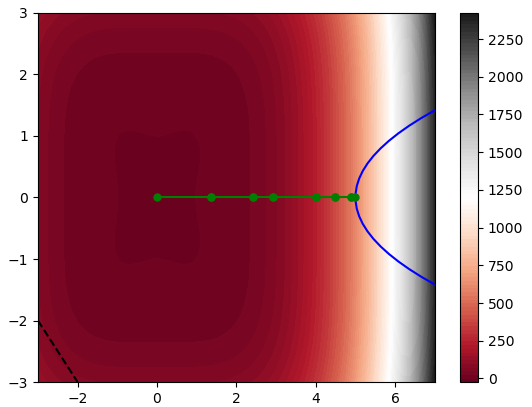
\includegraphics[width=\textwidth]{images/p_plot2.png}
    \caption{Kolejne kroki metody Powella-Gaussa-Seidela dla powyższego przykładu.}
    \label{uml_gauss_seidel}
\end{figure}
%comment
Spis kolejnych punktów, wartości funkcji celu oraz \textit{c}  dla $\epsilon_{1} = 10^{-1}$:
\begin{align*}
x &= [0, 0] & 
f(x) &= 5.00 &
c &= 5 \\
x &= [1.35761501133176, -5.42101086242752 * 10^{-20}] & 
f(x) &= 1.55396735606288 &
c &= 3.64238498866824 \\
x &= [2.41686096885252, -5.42101086242752 * 10^{-20}] & 
f(x) &= 28.2785984296559 &
c &= 2.58313903114748 \\
x &= [2.91569515573738, -5.42101086242752 * 10^{-20}] & 
f(x) &= 63.7704534929477 &
c &= 2.08430484426262 \\
x &= [4.00966300058885, -5.42101086242752 * 10^{-20}] & 
f(x) &= 242.405309081193 &
c &= 0.990336999411150 \\
x &= [4.48650306439799, -5.42101086242752 * 10^{-20}] & 
f(x) &= 385.036246326184 &
c &= 0.513496935602011 \\
x &= [4.89496898664932, -5.42101086242752 * 10^{-20}] & 
f(x) &= 550.155447682127 &
c &= 0.105031013350678 \\
x &= [4.98727223574502, -5.42101086242752 * 10^{-20}] & 
f(x) &= 593.787491705824 &
c &= 0.0127277642549837 \\
\end{align*}
%comment
Spis kolejnych punktów, wartości funkcji celu oraz \textit{c}  dla $\epsilon_{1} = 10^{-3}$:
\begin{align*}
x &= [0, 0] & 
f(x) &= 5.00 &
c &= 5 \\
x &= [1.35761501133176, -5.42101086242752 * 10^{-20}] & 
f(x) &= 1.55396735606288 &
c &= 3.64238498866824 \\
x &= [2.41686096885252, -5.42101086242752 * 10^{-20}] & 
f(x) &= 28.2785984296559 &
c &= 2.58313903114748 \\
x &= [2.91569515573738, -5.42101086242752 * 10^{-20}] & 
f(x) &= 63.7704534929477 &
c &= 2.08430484426262 \\
x &= [4.00966300058885, -5.42101086242752 * 10^{-20}] & 
f(x) &= 242.405309081193 &
c &= 0.990336999411150 \\
x &= [4.48650306439799, -5.42101086242752 * 10^{-20}] & 
f(x) &= 385.036246326184 &
c &= 0.513496935602011 \\
x &= [4.89496898664932, -5.42101086242752 * 10^{-20}] & 
f(x) &= 550.155447682127 &
c &= 0.105031013350678 \\
x &= [4.98727223574502, -5.42101086242752 * 10^{-20}] & 
f(x) &= 593.787491705824 &
c &= 0.012727764254983 \\
x &= [4.99826929728288,-5.42101086242752 * 10^{-20}] & 
f(x) &= 599.1524018694 &
c &= 0.001730702717123 \\
x &= [4.99913464864144,-5.42101086242752 * 10^{-20}] & 
f(x) &= 599.576089397458 &
c &= 0.000865351358562 \\
\end{align*}
%comment
\newline
\textbf{\textit{Szczegółowy opis techniki rozwiązania zadania:}} \\
Badania powyżej funkcji typu butelka, okazała się "trudna" dla algorytmu Powella ze względu na duży nakład obliczeń oraz liczbę kroków, które musiał ten algorytm wykonać. Dla prostych funkcji Powell wykona maksymalnie 3-5 kroków natomiast dla tak stromego zbocza jakim jest funkcja typu butelka, Powell wykonał dla $\epsilon_{1} = 10^{-1}$ odpowiednio 8 iteracji, a dla $\epsilon_{1} = 10^{-3}$ odpowiednio 11 iteracji. Natomiast algorytm poradził sobie z tego typu funkcją i odpowiednio znalazł minimum biorąc pod uwagę ograniczenia.

\subsubsection{Przykład III}
Funkcja celu:
\begin{equation}
    f(x_{1}, x_{2}) = (x_{1} - 2)^{2} + (x_{1} - x_{2}^{2})^{2}
\end{equation}
%comment
Ograniczenia:
\begin{equation}
    \begin{split}
        x_{1}^{2} + x_{2}^{2} - 1 &\leq 0
    \end{split}
\end{equation}
%comment
Parametry wejściowe:
\begin{align*}
    x &= [0; 0] & x &= [0; 0]\\
    \epsilon_{1} &= 10^{-1} & \epsilon_{1} &= 10^{-1} \\
    \epsilon_{2} &= 10^{-3} & \epsilon_{2} &= 10^{-3} \\
    \epsilon_{3} &= 10^{-3} & \epsilon_{3} &= 10^{-3} \\
    E &= 1 \mbox{ (długość kroku)} & E &= 5 \mbox{ (długość kroku)}\\
    L &= 1000 & L &= 1000
\end{align*}
%comment
\newpage
Rezultat w postaci warstwicy i zaznaczonych kolejnych kroków:
\begin{figure}[H]
    \centering
    \subfloat[\centering minimum pierwsze]{{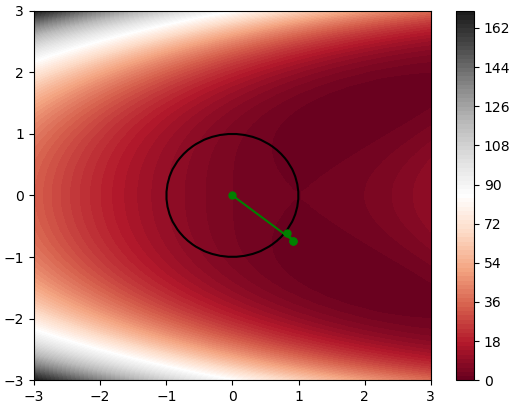
\includegraphics[width=0.47\textwidth]{images/p_plot3_e1.png} }}%
    \quad
    \subfloat[\centering minimum drugie]{{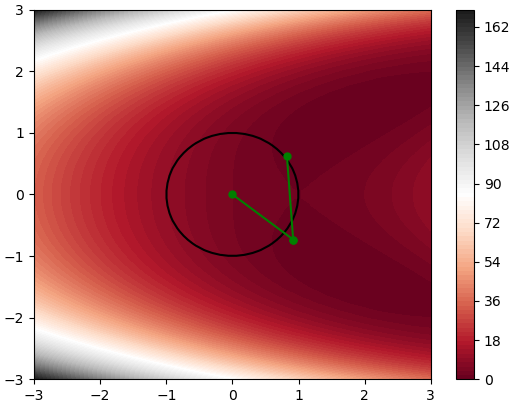
\includegraphics[width=0.47\textwidth]{images/p_plot3_e5.png} }}%
    \caption{Kolejne kroki metody Powella-Gaussa-Seidela dla powyższego przykładu.}
\end{figure}
%comment
Spis kolejnych punktów, wartości funkcji celu oraz \textit{c}  dla $\epsilon_{1} = 10^{-1}$ oraz $E = 1$:
\begin{align*}
x &= [0, 0] & 
f(x) &= 4.00 &
c &= 5 \\
x &= [0.919060381160095, -0.732962357484648] & 
f(x) &= 1.31422198430229 &
c &= 0.381905801707592 \\
x &= [0.824685111241693, -0.617300851314037] & 
f(x) &= 1.57816802447964 &
c &= 0.0611658737367592 \\
\end{align*}
%comment
Spis kolejnych punktów, wartości funkcji oraz \textit{c} celu dla $\epsilon_{1} = 10^{-1}$ oraz $E = 5$:
\begin{align*}
x &= [0, 0] & 
f(x) &= 4.00 &
c &= 5 \\
x &= [0.918856099415053, -0.733053715058343] & 
f(x) &= 1.31440549515172 &
c &= 0.381664280593084 \\
x &= [0.824720006729714, 0.617662597594127] & 
f(x) &= 1.57772075704230 &
c &= 0.0616701739669845 \\
\end{align*}
%comment
Spis kolejnych punktów, wartości funkcji oraz \textit{c} celu dla $\epsilon_{1} = 10^{-4}$ oraz $E = 1$:
\begin{align*}
x &= [0, 0] & 
f(x) &= 4.00 &
c &= 5 \\
x &= [0.919060381160095, -0.732962357484648] & 
f(x) &= 1.31422198430229 &
c &= 0.381905801707592 \\
x &= [0.824685111241693, -0.617300851314037] & 
f(x) &= 1.57816802447964 &
c &= 0.0611658737367592 \\
x &= [0.809610115019769, -0.596294648643902] & 
f(x) &= 1.62318294886841 &
c &= 0.0110358463436775 \\
x &= [0.806591030140483, -0.592369356057046] & 
f(x) &= 1.63187795914840 &
c &= 0.00149054389852549 \\
x &= [0.806957598858412, -0.591549683485333] & 
f(x) &= 1.63222345736340 &
c &= 0.00111159438693093 \\
x &= [0.806137926286698, -0.591916252203262] & 
f(x) &= 1.63303574846311 &
c &= 0.000223205820173489 \\
x &= [0.805771357568770, -0.592282820921190] & 
f(x) &= 1.63318195118940 &
c &= 0.0000664206365807440 \\
\end{align*}
%comment
Spis kolejnych punktów, wartości funkcji oraz \textit{c} celu dla $\epsilon_{1} = 10^{-4}$ oraz $E = 5$:
\begin{align*}
x &= [0, 0] & 
f(x) &= 4.00 &
c &= 5 \\
x &= [0.918856099415053, -0.733053715058343] & 
f(x) &= 1.31440549515172 &
c &= 0.381664280593084 \\
x &= [0.824720006729714, 0.617662597594127] & 
f(x) &= 1.57772075704230 &
c &= 0.0616701739669845 \\
x &= [0.809522441460765, 0.596203291070206] & 
f(x) &= 1.62341100356888 &
c &= 0.0107849475115424 \\
x &= [0.806824246512560, -0.592435463018399] & 
f(x) &= 1.63146255832803 &
c &= 0.00194514260238426 \\
x &= [0.806391570833279, 0.591467970787315] & 
f(x) &= 1.63314556851504 &
c &= 0.000101725978228440 \\
x &= [0.806824246512560,-0.591570111659838] & 
f(x) &= 1.63239770710439 &
c &= 0.000920561769792883 \\
x &= [0.806391570833279, 0.591467970787315] & 
f(x) &= 1.63314556851504 &
c &= 0.000101725978228329 \\
x &= [0.805958895153999, 0.591900646466596] & 
f(x) &= 1.63331692832089 &
c &= 0.0000838840345712688 \\
\end{align*}
%comment
\newline
\textbf{\textit{Szczegółowy opis techniki rozwiązania zadania:}} \\
W przykładzie tym analizujemy dokładnie tak samo jak w przypadku algorytmu \textit{Gaussa-Seidela} czy zmiana parametru długości kroku wpływa na poprawne działanie algorytmu, który zgodnie z oczekiwaniami znajdzie oba minima lokalne wraz z odpowiednią modyfikacją długości kroku. Odległość między dwoma minimami lokalnymi jest większa niż jeden. Tak więc przyjmując długość kroku $E = 1$ znajdujemy jedno z minimów lokalnych, natomiast zwiększając długość kroku $E = 5$ widzimy że Powell odpowiednio znajduje drugie minimum lokalne. Dla obu minimów został także bardzo radykalnie zmniejszy parametr $\epsilon_{1}$ do wartości $10^{-4}$ i jak widać z obliczeń, Powell także poradzi sobie numerycznie z tak dużym ograniczeniem.

\newpage
\subsection{Przykład własny}
Funkcja celu:
\begin{equation}
    f(x_{1}, x_{2}) = 2.5*(x_{1}^{2} - x_{2})^{2} + (1 - x_{1})^{2}
\end{equation}
%comment
\newline
Funkcja ta została zaczerpnięta z \cite{bibitem2}, strona 54, przykład 3.7.
\subsubsection{Gauss-Seidel}
%comment
%comment
Parametry wejściowe:
\begin{align*}
    x &= [-10; -10] \\
    \epsilon_{2} &= 10^{-3} \\
    \epsilon_{3} &= 10^{-3} \\
    E &= 5 \mbox{ (długość kroku)}\\
    L &= 1000
\end{align*}

%comment
Rezultat w postaci warstwicy i zaznaczonych kolejnych kroków:
\begin{figure}[H]
    \centering
    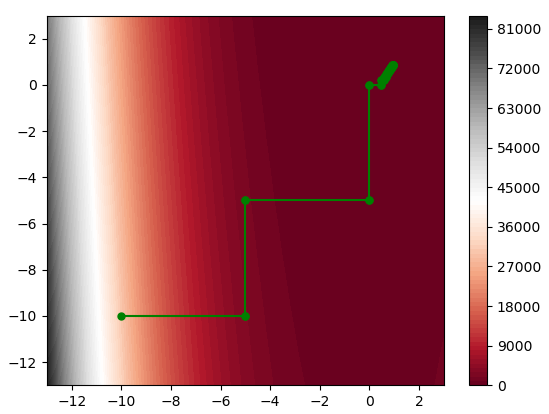
\includegraphics[width=\textwidth]{images/gs_plot4.png}
    \caption{Kolejne kroki metody Gaussa-Seidela dla powyższego przykładu.}
    \label{uml_gauss_seidel}
\end{figure}
%comment
\newpage
Spis kolejnych punktów i wartości funkcji celu:
\begin{align*}
x &= [-10, -10] & 
f(x) &= 30371.0000000000 \\
x &= [-5.00043267567928, -10] & 
f(x) &= 3099.26245430165 \\
x &= [-5.00043267567928, -5.00043267567928] & 
f(x) &= 2286.71919188236 \\
x &= [-0.000865351358561112, -5.00043267567928] & 
f(x) &= 63.5125675339985 \\
x &= [-0.000865351358561112, -0.000865351358561112] & 
f(x) &= 1.00173332687395 \\
x &= [0.471876349592011, -0.000865351358561112] & 
f(x) &= 0.403831693724519 \\
x &= [0.471876349592011, 0.222561397022101] & 
f(x) &= 0.278914618153198 \\
x &= [0.597399177235527, 0.222561397022101] & 
f(x) &= 0.207195020106014 \\
x &= [0.597399177235527, 0.356815766934554] & 
f(x) &= 0.162087434744140 \\
x &= [0.673741650576232, 0.356815766934554] & 
f(x) &= 0.130021383675323 \\
x &= [0.673741650576232, 0.454082730247378] & 
f(x) &= 0.106444570568096 \\
x &= [0.727224649482653, 0.454082730247378] & 
f(x) &= 0.0883838809300422 \\
x &= [0.727224649482653, 0.529025035677719] & 
f(x) &= 0.0744064635440676 \\
x &= [0.767979884134091, 0.529025035677719] & 
f(x) &= 0.0630652290098552 \\
x &= [0.767979884134091, 0.589839408942715] & 
f(x) &= 0.0538333395271616 \\
x &= [0.800003576516592, 0.589839408942715] & 
f(x) &= 0.0462902169307586 \\
x &= [0.800003576516592, 0.639987255476608] & 
f(x) &= 0.0399985702587265 \\
x &= [0.826096062450882, 0.639987255476608] & 
f(x) &= 0.0347470442946791 \\
x &= [0.826096062450882, 0.682473192845169] & 
f(x) &= 0.0302425831984893 \\
x &= [0.847657509847323, 0.682473192845169] & 
f(x) &= 0.0264572515791879 \\
x &= [0.847657509847323, 0.718493107213716] & 
f(x) &= 0.0232082365779903 \\
x &= [0.865883804871237, 0.718493107213716] & 
f(x) &= 0.0204303816862060 \\
x &= [0.865883804871237, 0.749651448237656] & 
f(x) &= 0.0179871804809447 \\
x &= [0.881514045819468, 0.749651448237656] & 
f(x) &= 0.0159179543130150 \\
x &= [0.881514045819468, 0.777144102082308] & 
f(x) &= 0.0140389361948966 \\
x &= [0.894674485753732, 0.777144102082308] & 
f(x) &= 0.0124504947965351 \\
x &= [0.894674485753732, 0.800436252195872] & 
f(x) &= 0.0110934640468227 \\
x &= [0.906104222970873, 0.800436252195872] & 
f(x) &= 0.00987614416924155 \\
x &= [0.906104222970873, 0.820928066488710] & 
f(x) &= 0.00881644036775962 \\
x &= [0.916133792277652, 0.820928066488710] & 
f(x) &= 0.00787746402780759 \\
x &= [0.916133792277652, 0.839154361512624] & 
f(x) &= 0.00703359464679015 \\
x &= [0.924763193674068, 0.839154361512624] & 
f(x) &= 0.00630318791242327 \\
x &= [0.924763193674068, 0.855115137267614] & 
f(x) &= 0.00566058992395896 \\
x &= [0.932527243711923, 0.855115137267614] & 
f(x) &= 0.00507761242151246 \\
x &= [0.932527243711923, 0.869675745112241] & 
f(x) &= 0.00455258463513092 \\
x &= [0.939425942391216, 0.869675745112241] & 
f(x) &= 0.00408172439016207 \\
x &= [0.939425942391216, 0.882505650239746] & 
f(x) &= 0.00366921705202562 \\
\end{align*}
%comment
\newpage
\textbf{\textit{Szczegółowy opis techniki rozwiązania zadania:}} \\
Badana funkcja posiada minimum lokalne, w przybliżeniu, w punkcie $x = [0.94, 0.88]$. Oczekiwaną wartością funkcji według \cite{bibitem2} powinna wynosić, w okolicy tego punktu $f(x_{1}, x_{2}) = 0$. Wartość ta została uzyskana, biorąc pod uwagę zadaną dokładność. Punkt startowy $x = [-10, -10]$ został specjalnie tak dobrany, aby pokazać wpływ długości kroku na liczbę iteracji. Jeżeli nie znamy minimum lokalnego warto, aby długość kroku była bardzo dużą liczbą, ponieważ możemy zaoszczędzić algorytmowi wielu iteracji, aż do pożądanego punktu. W ten sposób algorytm \textit{Gaussa-Seidela} wykona tylko i wyłącznie dwa kroki w pobliże minimum lokalnego.

\subsubsection{Powell-Gauss-Seidel}
Ograniczenia:
\begin{equation}
    \begin{split}
        x_{1}^{2} + x_{2}^{2} - 0.5 &\leq 0 \\
        (x_{1} + 1)^{2} + x_{2}^{2} - 0.5 &\leq 0 \\
        (x_{1} + 0.5)^{2} + (x_{2} + 1)^{2} - 0.5 &\leq 0 \\
    \end{split}
\end{equation}
%comment
Ograniczenia zostały dobrane przez Nas w taki sposób, aby uzyskać przecięcie trzech niedużych okręgów oddalonych od minimum lokalnego. Chcieliśmy uzyskać bardzo mały obszar rozwiązań dopuszczalnych, aby sprawdzić czy poradzi sobie algorytm \textit{Powella-Gaussa-Seidela}. Rezultat w postaci warstwicy i zaznaczonych kolejnych kroków:
\begin{figure}[H]
    \centering
    \subfloat[\centering $\epsilon_{1} = 10^{-1}$]{{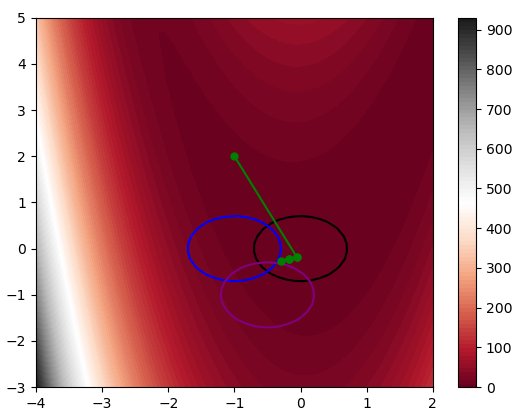
\includegraphics[width=0.47\textwidth]{images/p_plot4_c=0.1.png} }}%
    \quad
    \subfloat[\centering $\epsilon_{1} = 10^{-3}$]{{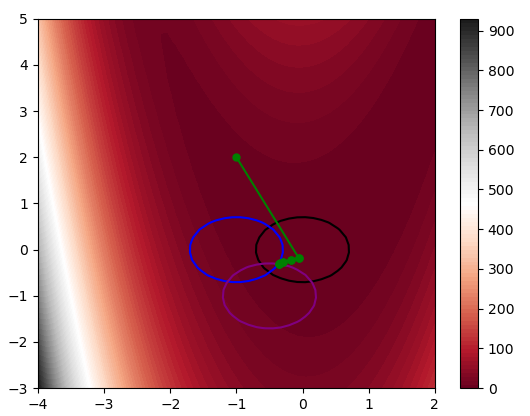
\includegraphics[width=0.47\textwidth]{images/p_plot4_c=0.001.png} }}%
    \caption{Kolejne kroki metody Powella-Gaussa-Seidela dla powyższego przykładu.}
\end{figure}
%comment
Spis kolejnych punktów, wartości funkcji celu oraz \textit{c}  dla $\epsilon_{1} = 10^{-1}$ oraz $E = 5$:
\begin{align*}
x &= [-1, 2] & 
f(x) &= 6.50 &
c &= 5 \\
x &= [-0.0585128200849023, -0.179408429179035] & 
f(x) &= 1.20401840474696 &
c &= 0.418585494404973 \\
x &= [-0.181667987586973, -0.218661355047589] & 
f(x) &= 1.55467692617882 &
c &= 0.217480070731202 \\
x &= [-0.302227101013360, -0.274842548902215] & 
f(x) &= 2.03102180520688 &
c &= 0.0649674484562159 \\
\end{align*}
%comment
Spis kolejnych punktów, wartości funkcji celu oraz \textit{c}  dla $\epsilon_{1} = 10^{-3}$ oraz $E = 5$:
\begin{align*}
x &= [-1, 2] & 
f(x) &= 6.50 &
c &= 5 \\
x &= [-0.0585128200849023, -0.179408429179035] & 
f(x) &= 1.20401840474696 &
c &= 0.418585494404973 \\
x &= [-0.181667987586973, -0.218661355047589] & 
f(x) &= 1.55467692617882 &
c &= 0.217480070731202 \\
x &= [-0.302227101013360, -0.274842548902215] & 
f(x) &= 2.03102180520688 &
c &= 0.0649674484562159 \\
x &= [-0.341480026881914, -0.294036336157211] & 
f(x) &= 2.22114183948676 &
c &= 0.0235132765436926 \\
x &= [-0.358943111419788, -0.304498581143271] & 
f(x) &= 2.31618253552503 &
c &= 0.00367332031440731 \\
x &= [-0.362939333405835, -0.305898749053634] & 
f(x) &= 2.33638990277532 &
c &= 0.00057966240601972 \\
\end{align*}
%comment
\textbf{\textit{Szczegółowy opis techniki rozwiązania zadania:}} \\
Punkt początkowy został specjalnie dobrany w taki sposób, aby było z poza obszaru dozwolonych rozwiązań, aby zobaczyć jak poradzi sobie algorytm \textit{Powella-Gaussa-Seidela}. Powell nie musi mieć punktu początkowego w dozwolonym obszarze rozwiązań, wtedy będzie się kierował w stronę obszaru ograniczeń. Niezależnie od parametru $\epsilon_{1}$ można zauważyć, że po pierwszym kroku Powell znajduje się bardzo blisko dostępnego obszaru rozwiązań. Następnie w zależności od pożądanej dokładności kieruje się dokładnie w linii prostej do dopuszczalnego obszaru rozwiązań. Dla $\epsilon_{1} = 10^{-3}$ możemy zauważyć, że punkt końcowy znajduje się dokładnie na przecięciu okręgów niebieskiego i fioletowego, wewnątrz okręgu czarnego. Warto też zauważyć, że po pierwszym kroku wartość funkcji celu była mniejsza niż w ostatnim, z dopuszczalnego obszaru rozwiązań. Pokazuje to, że metoda przesuwanej kary Powella została poprawnie zaimplementowana, a sam algorytm zawsze dąży do obszaru dozwolonych rozwiązań. 

\subsection{Wpływ punktu początkowego na szybkość działania algorytmu}
Zakładając, że funkcja, którą minimalizujemy nie posiada bardzo stromego zbocza to najbardziej istotnym parametrem wpływającym na szybkość działania algorytmu, a doborem punktu początkowego jest długość kroku przyjęta przez metodę \textit{Gaussa-Seidela}, która oblicza przedział poszukiwań, który jest następnie przekazywany do metody \textit{Złotego Podziału}. Jeżeli wartość długości kroku będzie mała to metoda \textit{Gaussa-Seidela} będzie niepotrzebnie iterować, gdyż \textit{Złoty Podział} mógłby wykonywać dłuższe kroki dochodząc w ten sposób szybciej do szukanego obszaru. W przypadku funkcji, która ma bardzo strome zbocze, dobór odpowiedniego punktu początkowego jest bardzo ważny, ponieważ z innym przypadku może się okazać, że algorytm zakończy działanie dochodząc do maksymalnej liczby iteracji lub z powodu braku zasobów jak pamięć operacyjna. W tym przypadku istotne może się okazać zmniejszenie dokładności poszukiwanego minimum dla metody \textit{Gaussa-Seidela} i dobranie tak punktu początkowego, aby algorytm nie musiał przechodzić przez całe zbocze. Podsumowując, w zależności od badanej funkcji celu, trzeba mieć na uwadze, że nieodpowiednie dobranie punktu początkowego lub zbyt duża dokładność, może sprawić, że algorytm będzie wykonywał się bardzo długo lub też braknie mu zasobów jak pamięć operacyjna.

\newpage
\section{Wnioski}
\begin{enumerate}
    \item Projekt pierwotnie wydawał się bardzo trudny. Problemem okazało się także znalezienie fachowej literatury, która opisywałaby wszystkie interesujące Nas metody. Dzięki literaturze \cite{bibitem1} w dużej mierze wszystkie metody okazały się łatwe ze względu na bardzo dokładny opis każdego z kroków algorytmu wraz z ilustracjami, prezentującymi przykładowe działanie.
    
    \item Sam projekt okazał się bardzo interesujący, ponieważ mieliśmy zaimplementować i przetestować trzy różne metody, a następnie złożyć te metody w jedną całość:
    \begin{itemize}
        \item \textit{Złoty Podział}
        \item \textit{Gauss-Seidel}
        \item \textit{Powell}
    \end{itemize}
    Kluczowe okazało się implementowanie i testowanie metody za metodą. Najpierw naturalnie została zaimplementowana metoda minimum w kierunku \textit{Złoty Podział} i przetestowana na przykładzie z literatury \cite{bibitem2}. Następnie została zaimplementowana metoda minimalizacji funkcji \textit{Gaussa-Seidela} i również przetestowana na przykładach. W tym momencie mieliśmy pewność, że poprawnie zaimplementowany Powell musi działać poprawnie, ponieważ zarówno \textit{Gauss-Seidel} oraz \textit{Złoty Podział} działały dobrze. Tak więc złożenie tych trzech metod nie stanowiło większego problemu, gdyż wcześniej zostały dobrze przetestowane.
    
    \item Bardzo przydatne w przypadku przesuwanej funkcji kary Powella okazało się przeniesienie kroków algorytmu z literatury \cite{bibitem1} na schemat blokowy. Dzięki temu implementacja samej metody była bardzo prosta, ponieważ wizualnie można było zobaczyć wszystkie zależności w algorytmie.
    
    \item Po zaimplementowaniu i przetestowaniu metod \textit{Złotego Podziału} oraz \textit{Gaussa-Seidela} bardzo ważne okazały się analityczne obliczenia na kartce metody przesuwanej funkcji kary Powella. Pozwoliło Nam to poznać dogłębnie sens i zasadzę działania algorytmu. Dzięki temu mogliśmy później testować sam program, mając pod ręką obliczenia na kartce.
    
    \item Kluczowe w testowaniu algorytmów \textit{Powella} czy \textit{Gaussa-Seidela} okazały się funkcje celu, które miały więcej niż jedno minimum. Pozwoliło to sprawdzić czy przy odpowiednim doborze długości kroku, poszukiwane minima zostaną znalezione. Dodatkowo wypisanie na ekran uzyskanych punktów jak i wyrysowanie ich, umożliwiało weryfikację, czy algorytm odpowiednio reaguje na zwiększenie dokładności obliczeń poprzez modyfikację: $\epsilon_{1}$, $\epsilon_{2}$, $\epsilon_{3}$.
    
    \item Ważny był również odpowiedni wybór środowiska programistycznego, które udostępnia cały wachlarz bibliotek umożliwiające skupienie się na algorytmach, a nie rzeczach pobocznych. Wybór \textit{Pythona} okazał się trafny, ponieważ posiadał kluczowe biblioteki umożliwiające parsowanie, obliczanie równań, efektywne operacje na wektorach i macierzach, rysowanie wykresów jak i nanoszenie ograniczeń lub kolejnych kroków algorytmu, a także prosty framework do implementacji interfejsu graficznego z wieloma poradnikami.
    
    \item Z punktu widzenia studenckiego, ważne było, aby sumiennie konsultować się z prowadzącą zajęcia, by zrozumieć matematykę, za pomocą której opisane są algorytmy lub wytłumaczyć niejasności, jak i sumienna praca nad realizacją programistyczną projektu.
\end{enumerate}

\newpage
\section{Bibliografia}
\begin{thebibliography}{3}
    \bibitem{bibitem1} 
    Władysław Findeisen, Jacek Szymanowski i Andrzej Wierzbicki. \\
    \textit{Metody Obliczeniowe Optymalizacji}. \\
    Warszawa 1972.
    
    \bibitem{bibitem2}
    Jan Kusiak, Anna Danielewska-Tułecka i Piotr Oprocha. \\
    \textit{Optymalizacja. Wybrane metody z przykładami zastosowań.} \\
    PWN Warszawa 2019.
    
    \bibitem{bibitem3}
    Jacek Stadnicki. \\
    \textit{Teoria i praktyka rozwiązywania zadań optymalizacji.} \\
    PWN Warszawa 2017.
\end{thebibliography}

\end{document}
